\documentclass{article}

\makeatletter
\renewcommand{\fnum@figure}{Εικόνα \thefigure}
\makeatother

\usepackage[greek, english]{babel}
\usepackage{alphabeta}
\usepackage{atbegshi, picture}

% Set page size and margins
% Replace `letterpaper' with`a4paper' for UK/EU standard size
\usepackage[letterpaper,top=2cm,bottom=2cm,left=3cm,right=3cm,marginparwidth=1.75cm]{geometry}

% Useful packages
\usepackage{amsmath}
\usepackage{graphicx}
\usepackage[colorlinks=true, allcolors=blue]{hyperref}
\usepackage[utf8]{inputenc}
\usepackage{indentfirst}

\newcommand\T{\rule{0pt}{2.6ex}}       % Top strut
\newcommand\B{\rule[-1.2ex]{0pt}{0pt}} 


\addto\captionsenglish{
  \renewcommand{\contentsname}
    {Περιεχόμενα}
}

% \title{Feasibility Study}
% \date{}

\begin{document}
% \maketitle

\begin{titlepage}
   \begin{center}
       \vspace*{1cm}

       \textbf{\huge Use Cases}

       \vspace{0.5cm}
        Τεχνολογία Λογισμικού
            
       \vspace{1cm}

       \textbf{Κατερίνα Μητροπούλου\\Στεφανίδης Μάριος}
       
       \begin{figure}[!htb]
        \centering
        
\includegraphics[width=0.5\textwidth]{logo.png}
        \end{figure}
        
        \vspace{0.5cm}
        
        \begin{figure}[!htb]
        \centering
        \includegraphics[width=0.5\textwidth]{UoP.jpg}
        \end{figure}


       \vfill
            
       Τεχνικό Κείμενο για την Τεχνολογία Λογισμικού\\
            
       \vspace{0.5cm}
            
       CEID, ECE\\
       University of Patras\\
            
   \end{center}
\end{titlepage}


 \noindent Η ομάδα μας

\begin{enumerate}
  \item Βεργίνης Δημήτριος, ΑΜ: 1066634 , ECE
  \item Βλαχογιάννης Δημήτριος, ΑΜ: 1067371, CEID
  \item Κούρου Αγγελική, ΑΜ: 1067499 , CEID
  \item Μητροπούλου Αικατερίνα - Quality Manager, ΑΜ: 1067409, CEID
  \item Στεφανίδης Μάριος - Project Manager, ΑΜ:1067458, CEID
\end{enumerate}

{
  \hypersetup{linkcolor=black}
  \tableofcontents
}

\newpage

\section{Εισαγωγή}

Τα Use Cases αποτελούν ένα σύνολο δραστηριοτήτων ή βημάτων που λαμβάνουν χώρα κατά την πλοήγηση ενός χρήστη (ή ρόλου, γνωστού στην UML ως ηθοποιού) σε ένα σύστημα, για να επιτευχθεί ένας στόχος. Ο ηθοποιός μπορεί να είναι άνθρωπος ή κάποιο άλλο εξωτερικό σύστημα. 
Για την ανάπτυξη ενός use case χρησιμοποιούνται τα διαγράμματα περιπτώσεων χρήσης, καθώς και λεκτική περιγραφή των περιπτώσεων αυτών.

\section{Διάγραμμα Περιπτώσεων Χρήσης}

Παρακάτω παρουσιάζεται το διάγραμμα περιπτώσεων χρήσης. Για την καλύτερη κατανόηση του διαγράμματος σημειώνεται ότι:

\begin{enumerate}
  \item Τα σκίτσα με τους ανθρώπους αντιστοιχούν στους ηθοποιούς του εκάστοτε use case, δηλαδή τους εμπλεκόμενους
  \item Οι μπλε ελλείψεις αντιστοιχούν στα use cases
  \item Οι μαύρες γραμμές απεικονίζουν άμεση συσχέτιση μεταξύ ενός ηθοποιού και μίας περίπτωσης χρήσης
  \item Οι μπλε διακεκομμένες γραμμές (το μπλε επιλέχθηκε για ευαναγνωσία) απεικονίζουν τη σχέση εξάρτησης μεταξύ δύο περιπτώσεων χρήσης, δηλαδή το use case στο οποίο δείχνει το βέλος δεν μπορεί να υπάρξει αν δεν έχει προηγηθεί το use case από το οποίο ξεκινάει το βέλος  
\end{enumerate}


\underline{Σημείωση}: Στο παρακάτω διάγραμμα, ενώ το use case που αφορά στην διαδικασία log in, είναι προαπαιτούμενο για την ύπαρξη όλων των υπολοίπων, δεν παριστάνονται οι συγκεκριμένες συσχετίσεις εξάρτησης για την καλύτερη παρουσίαση και ευαναγνωσία του διαγράμματος.
\par Ακόμα, η λειτουργία cancel παρουασιάζεται ενδεικτικά σε κάποια από τα παρακάτω σενάριο χρήσης και όχι σε όλα όσα μπορεί να εφαρμοστεί για να αποφευχθεί η συνεχής επανάληψή της και να παρουσιαστούν κι άλλες λειτουργίες του συστήματος.

\newpage

\begin{figure}[!htb]
        \centering
        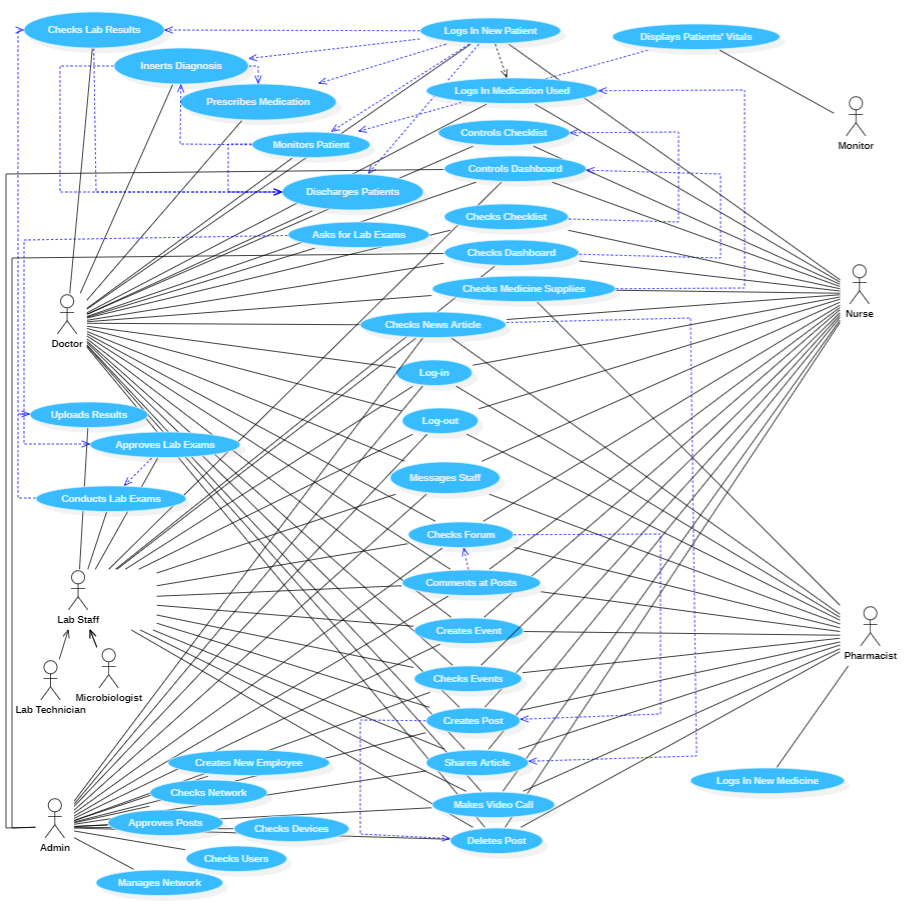
\includegraphics[width=1.1\textwidth]{UML.png}
        \caption{\label{fig: UML} Use Case Diagram}
\end{figure}
        
\vspace{0.5cm}

Για τις παρακάτω περιπτώσεις χρήσης δεν αναγράφονται στους πίνακες τα παρακάτω ως \par προαπαιτούμενα χάριν συντομίας:

\begin{enumerate}
    \item  Ο εκάστοτε "ηθοποιός" έχει καταχωρηθεί στο σύστημα
    \item Ο "ηθοποιός" έχει συνδεθεί στο \textbf{Medic World}
\end{enumerate}

\newpage

\section{Use Case 1: Ενέργειες στην Καρτέλα Ασθενούς}

Παρακάτω θα αναλυθεί το σενάριο χρήσης του \textbf{Medic World}, στο οποίο ένας γιατρός πραγματοποιεί συγκεκριμένες αλλαγές στην καρτέλα ενός ασθενούς.

\subsection{Γενική Περιγραφή}

Εξαιτίας του γεγονότος ότι οι λειτουργίες που μπορούν να πραγματοποιηθούν μέσω της καρτέλα του ασθενούς είναι πολυάριθμες, αποφασίσαμε να αναλύσουμε δύο απο τις πιο σημαντικές, την εισαγωγή διάγνωσης και την έκδοση εξιτηρίου.
\par Καθώς τα βήματα των συγκεκριμένων περιπτώσεων χρήσης ως ένα σημείο ταυτίζονται, παρακάτω θα παρουσιαστεί ένας κοινός πίνακας με τα βήματα που είναι ίδια και για τα δύο και στη συνέχεια θα χωριστούν σε δύο διαφορετικά use cases. 

 \subsection{Γενικό Σενάριο Χρήσης}
 
 \begin{center}
     \begin{tabular}{|l|l|}
     \hline
      \textbf{Βήμα 1} & Ο γιατρός από το κεντρικό μενού επιλέγει να μεταφερθεί στις \T \\& καρτέλες των ασθενών \B \\
      \hline
      \textbf{Βήμα 2} &  Στο νέο παράθυρο το σύστημα εμφανίζει όλους τους ενεργούς ασθενείς \T \\& που νοσηλεύονται στο νοσοκομείο \B \\
      \hline
      \textbf{Βήμα 3} & Στο ίδιο παράθυρο επιλέγει τον ασθενή που χρειάζεται διάγνωση \T\B \\
      \hline
      \textbf{Βήμα 4} & Σε νέο παράθυρο εμφανίζονται οι τρέχουσες ζωτικές ενδείξεις του ασθενούς, \T \\& τα συμπτώματα του, αποτελέσματα από την ψιλάφιση/εξέταση, η ομάδα γιατρών \\& που τον παρακολουθεί, οι αλλεργίες του κ.ο.κ. \B \\
      \hline
      \textbf{Βήμα 5} & Ο γιατρός επιθμεί να ελέγξει το ιστορικό του ασθενούς \T\B \\
      \hline
      \textbf{Βήμα 6} & Σε νέα καρτέλα το σύστημα εμφανίζει τα δημογραφικά και κλινικά δεδομένα του \T\B \\
      \hline
      \textbf{Βήμα 7} & Είναι έτοιμος να συμπληρώσει τη διάγνωση/να εκδόσει το εξιτήριο \T\B \\
      \hline      
     
     \end{tabular}
 \end{center}
 
\textbf{\underline{Εναλλακτική Ροή 1}:} \vspace{0.2cm}
\par \textbf{Βήμα 3.1.α:} Στην μπάρα αναζήτησης πληκτρολογεί το όνομα του ασθενούς και το σύστημα \par εμφανίζει προτάσεις με ασθενείς που είναι ήδη καταχωρημένοι και έχουν παρόμοιο όνομα με αυτό που \par πληκτρολογεί ο γιατρός.\vspace{0.1cm} 
\par Τα υπόλοιπα βήματα ταυτίζονται με τα βήματα 4 έως 7 της κανονικής ροής.

\vspace{0.2cm}

\par \textbf{Βήμα 3.1.β:}  Πληκτρολογεί το όνομα του ασθενούς και στην μπάρα αναζήτησης το σύστημα δεν \par εμφανίζει προτάσεις με ασθενείς που έχουν παρόμοιο όνομα με αυτό που πληκτρολογεί ο γιατρός. \vspace{0.1cm}
\par \textbf{Βήμα 4.1.β:} Το σύστημα εμφανίζει μήνυμα ότι δεν υπάρχει ασθενής με όνομα παρόμοιο με αυτό \par που αναζητεί ο γιατρός. \vspace{0.1cm}
\par \textbf{Βήμα 5.1.β:} Το σύστημα κλείνει την μπάρα αναζήτησης και εμφανίζει την οθόνη με τις καρτέλες \par των ασθενών. \vspace{0.1cm}

\par Τα υπόλοιπα βήματα ταυτίζονται με τα βήματα 4 έως 7 της κανονικής ροής. 

\newpage

\subsubsection{Εισαγωγή Διάγνωσης}
 
 \begin{center}
     \begin{tabular}{|l|l|}
     \hline
      \textbf{Περίπτωση Χρήσης 1.1} & Ο γιατρός εισάγει τη διάγνωση ενός ασθενούς \T\B \\ 
      \hline
      \textbf{Ηθοποιός} & Γιατρός \T\B \\
      \hline
      \textbf{Σενάριο Περίπτωσης Χρήσης} & Ένας από τους ασθενείς χρείαζεται διάγνωση, οπότε \T\\& ο γιατρός εισέρχεται στην καρτέλα του, μελετάει τα\\& αποτελέσματα των εξετάσεών και τα συμπτώματά του και \\& καταλήγει σε διάγνωση \B \\
      \hline
      \textbf{Αφορμή} & Ασθενής χρειάζεται διάγνωση \T\B \\
      \hline
      \textbf{Προαπαιτούμενο 1} & Να έχει καταχωρηθεί ο ασθενής στο σύστημα \T\B \\
      \hline
      \textbf{Προαπαιτούμενο 2} & Να είναι έτοιμα τα αποτελέσματα των εργαστηριακών εξετάσεων \T\B \\
      \hline
     \end{tabular}
 \end{center}
 
  \vspace{0.2cm}
 
 \begin{center}
     \begin{tabular}{|l|l|}
     \hline
      \textbf{Περιγραφή} & Αυτό το σενάριο περιγράφει μια κατάσταση όπου χρειάζεται \T \\& η πλοήγηση σε τέσσερις καρτέλες, οι οποίες τελικά\\& οδηγούν στην επίτευξη του στόχου. \B \\ 
      \hline
      \textbf{Βήμα 8} & Στην ίδια οθόνη το σύστημα εμφανίζει σε αναδυόμενο παράθυρο μια λίστα με \T \\& πιθανές προτάσεις ασθενειών που ταιριάζουν στο προφίλ του ασθενούς \\& σύμφωνα με τα συμπτώματα και τις εξετάσεις του \B \\
      \hline
      \textbf{Βήμα 9} & Ο γιατρός επιλέγει την ασθένεια που ταυτίζεται με τη διάγνωσή του  \T\B \\
      \hline
      \textbf{Βήμα 10} & Σε νέα καρτέλα εμφανίζεται η προεπισκόπηση της διάγνωσης \T\B \\
      \hline
      \textbf{Βήμα 11} & Ο γιατρός καταχωρεί την διάγνωση του \T\B \\
      \hline
      \textbf{Βήμα 12} & Σε αναδυόμενο παράθυρο εμφανίζεται μήνυμα επιτυχίας \T\B \\
      \hline    
      \textbf{Βήμα 13} & Επιλέγει την ένδειξη "ΟΚ" \T\B \\ 
      \hline
      \textbf{Βήμα 14} & Ενημερώνεται το σύστημα και το προφίλ του ασθενούς \T\B \\
      \hline
    \end{tabular}
 \end{center}
 
  \textbf{\underline{Εναλλακτική Ροή 1}:}  \vspace{0.2cm}
\par \textbf{Βήμα 9.1.:} Δεν τον ικανοποιεί καθόλου η λίστα των πιθανών ασθενειών, επομένως \par "κλείνει" αυτό το παράθυρο. \vspace{0.1cm}
\par \textbf{Βήμα 10.1:} Κατευθύνεται απευθείας στο παράθυρο προεπισκόπησης της διάγνωσης. \vspace{0.1cm}
\par \textbf{Βήμα 11.1:} Εισάγει τη διάγνωση του. \vspace{0.1cm}

\par Τα υπόλοιπα βήματα ταυτίζονται με τα βήματα 11 έως 14 της κανονικής ροής.

\vspace{0.2cm}

\textbf{\underline{Εναλλακτική Ροή 2}:}  \vspace{0.2cm}
\par \textbf{Βήμα 11.2:} Ο Γιατρός τροποποιεί την διάγνωση, εφόσον δεν τον ικανοποιεί πλήρως η πρόταση \par του συστήματος και επιθυμεί να συμπληρώσει κάτι. \vspace{0.1cm}

\par Τα υπόλοιπα βήματα ταυτίζονται με τα βήματα 11 έως 14 της κανονικής ροής.\vspace{0.1cm}

\newpage

 \subsubsection{Έκδοση Εξιτηρίου}
 
 \begin{center}
     \begin{tabular}{|l|l|}
     \hline
      \textbf{Περίπτωση Χρήσης 1.2} & Ο γιατρός δίνει εξιτήριο σε κάποιον ασθενή \T\B \\ 
      \hline
      \textbf{Ηθοποιός} & Γιατρός \T\B \\
      \hline
      \textbf{Σενάριο Περίπτωσης Χρήσης} & Ένας από τους ασθενής ολοκλήρωσε τη θεραπεία του, οπότε \T\\& ο γιατρός εισέρχεται στην καρτέλα του για να του δώσει εξιτήριο \B \\
      \hline
      \textbf{Αφορμή} & Ασθενής χρειάζεται εξιτήριο \T\B \\
      \hline
      \textbf{Προαπαιτούμενο 1} & Να έχει καταχωρηθεί ο ασθενής στο σύστημα \T\B \\
      \hline
     \end{tabular}
 \end{center}
 
 \vspace{0.2cm}
 \begin{center}
     \begin{tabular}{|l|l|}
     \hline
      \textbf{Περιγραφή} & Αυτό το σενάριο περιγράφει μια κατάσταση όπου χρειάζεται \T \\& πλοήγηση σε τρεις καρτέλες, οι οποίες οδηγούν στην επίτευξη \\& του στόχου \B \\ 
      \hline
      \textbf{Βήμα 8} & Σε νέο παράθυρο ο γιατρός συμπληρώνει τα απαραίτητα στοιχεία της φόρμας \T \\& εξιτηρίου (medication και nutrition recommendations) \\
      \hline
      \textbf{Βήμα 9} & Επιθυμεί να εκτυπώσει τη συγκεκριμένη φόρμα \T\B \\
      \hline
      \textbf{Βήμα 10} & Σε αναδυόμενο παράθυρο εμφανίζεται το pdf αρχείο \T \\& του εξιτηρίου και οι διάφορες λειτουργίες/επιλογές εκτύπωσης \\& (π.χ. εύρεση κοντινών εκτυπωτών) \B \\
      \hline
      \textbf{Βήμα 11} & Αφού επιλέξει κάποιον από τους κοντινούς εκτυπωτές, \T \\& δίνει έγκριση για εκτύπωση και όταν αυτή ολοκληρωθεί, \\& εμφανίζεται μήνυμα επιτυχίας \B \\
      \hline
      \textbf{Βήμα 12} & Επιστρέφει στο παράθυρο "Post-discharge Guidance" από το οποίο επιθυμεί να \T \\& κοινοποιήσει μέσω ηλεκτρονικού ταχυδρομείου τις οδηγίες εξιτηρίου \B \\
      \hline
      \textbf{Βήμα 14} & Σε νέο παράθυρο εμφανίζεται το εξιτήριο σε pdf μορφή από το οποίο \T\\&επιβεβαίωνει την κοινοποίηση του \B \\
      \hline
      \textbf{Βήμα 15} & Στέλνεται αυτομάτως μήνυμα στο email που έχει καταχωρηθεί \T \\& για τον συγκεκριμένο ασθενή και εμφανίζεται μήνυμα επιτυχίας \B \\
      \hline
      \textbf{Βήμα 16} & Επιστρέφει στο παράθυρο "Post-discharge Guidance" και \T \\& επιβεβαίωνει την έκδοση του εξιτηρίου  \B \\   
      \hline
      \textbf{Βήμα 17} & Εμφανίζεται μήνυμα επιτυχίας και ενημερώνονται κατάλληλα \T \\& οι καρτέλες ασθενών  \B \\      
      \hline
     \end{tabular}
 \end{center}
 
 \textbf{\underline{Εναλλακτική Ροή 1}:} \vspace{0.2cm}
\par \textbf{Βήμα 15.1:} Δεν έχει καταχωρηθεί e-mail για τον συγκεκριμένο ασθενή, συνεπώς οδηγείται σε \par αναδυόμενο παράθυρο, το οποίο ζητά από τον γιατρό την συμπλήρωση κάποιας διεύθυνσης \par ηλεκτρονικού ταχυδρομείου.

\vspace{0.2cm}

\par \textbf{Βήμα 16.1.α:} Ο Γιατρός εισάγει ένα email που πληροί τις προυϋποθέσεις και επιβεβαιώνει την \par καταχώρηση. \vspace{0.2cm}
\par \textbf{Βήμα 16.1.β:} Το email είναι λανθασμένο (δεν έχει τη μορφή ...@...com) και το σύστημα κλειδώνει \par την λειτουργία επιβεβαίωσης καταχώρησης εώς ότου εισαχθεί σωστό email. \vspace{0.1cm}

\par *Αντίστοιχη διαδικασία με το βήμα 16.1.β ακολουθείται, εάν η διεύθυνση ταχυδρομίου που συμπληρω- \parθεί δεν είναι έγκυρη (λ.χ. δεν υπάρχει ο συγκεκριμένος λογαριασμός).

\par Τα υπόλοιπα βήματα ταυτίζονται με τα βήματα 15 και 17 της κανονικής ροής.

\vspace{0.2cm}

\textbf{\underline{Εναλλακτική Ροή 2}:} \vspace{0.2cm}
\par \textbf{Βήμα 10.2/Βήμα 14.2:} Ο διαχειριστής επιθυμεί την ακύρωση της διαδικασίας.

\vspace{0.3cm}

\par \textbf{Βημα 11.2.α/Βήμα 15.2.α:} Εμφανίζεται νέο παράθυρο για την επιβεβαίωση της "ακύρωσης". \vspace{0.1cm}
\par \textbf{Βημα 12.2.α/Βήμα 16.2.α:} Επιβεβαιώνει την "ακύρωση". \vspace{0.1cm}
\par \textbf{Βημα 13.2.α/Βήμα 17.2.α:} Επιστρέφει στην προηγούμενη καρτέλα (post discharge guide) \vspace{0.3cm}

\par \textbf{Βημα 14.2.β/Βήμα 16.2.β:}  Απορρίπτει την "ακύρωση". \vspace{0.1cm}
\par \textbf{Βημα 15.2.β/Βήμα 17.2.β:} Επιστρέφει στην καρτέλα που βρισκόταν.

\section{Use Case 2: Καταχώρηση Νέου Φαρμάκου }
 
 Παρακάτω θα αναλυθεί το σενάριο χρήσης του \textbf{Medic World} κατά το οποίο ένας φαρμακοποιός επιθυμεί να εισάγει στο σύστημα ένα νέο φάρμακο.
 
\subsection{Περιγραφή}

\begin{center}
     \begin{tabular}{|l|l|}
     \hline
      \textbf{Περίπτωση Χρήσης 3} & Ο χρήστης εισάγει νέο φάρμακο στην καρτέλα προμηθειών \T\B \\ 
      \hline
      \textbf{Ηθοποιός} & Φαρμακοποιός \T\B \\
      \hline
      \textbf{Σενάριο Περίπτωσης Χρήσης} & Έχει γίνει από το νοσοκομείο αγορά ενός νέου φαρμάκου \T \\& και ο φαρμακοποιός καλείται να το καταχωρήσει \\& στην καρτέλα προμηθειών \B \\
      \hline
      \textbf{Αφορμή} & Η αγορά νέου φαρμάκου \T\B \\
      \hline
      \textbf{Προαπαιτούμενο 1} &  Να μην υπάρχει ήδη το φάρμακο στην καρτέλα προμηθειών \T\B \\
      \hline
     \end{tabular}
 \end{center}
 
  \subsection{Αναλυτικό Σενάριο Χρήσης}
 
 \begin{center}
     \begin{tabular}{|l|l|}
     \hline
      \textbf{Περιγραφή} & Αυτό το σενάριο περιγράφει μια κατάσταση όπου χρειάζεται \T \\& πλοήγηση σε δύο καρτέλες, οι οποίες οδηγούν στην επίτευξη \\& του στόχου \B \\ 
      \hline
      \textbf{Βήμα 1} & Ο φαρμακοποιός από το κεντρικό μενού επιλέγει να μεταφερθεί στην \T \\& καρτέλα των προμηθειών \B \\
      \hline
      \textbf{Βήμα 2} & Στο νέο παράθυρο το σύστημα εμφανίζει όλες τις διαθέσιμες κατηγορίες \T \\& φαρμάκων του νοσοκομείου εκείνη την στιγμή \B \\
      \hline
      \textbf{Βήμα 3} & Στο ίδιο παράθυρο ο χρήστης επιλέγει την λειτουργεία "New Medicine" \T \\& (προσθήκη νέου φαρμάκου) \B \\
      \hline
      \textbf{Βήμα 4} & Σε νεό παράθυρο εμφανίζονται όλα τα πεδία που πρέπει να συμπληρώσει \T \\&  ο φαρμακοποιός για την καταχώριση νέου φαρμάκου. Πληκτρολογώντας τη \\& κατηγορία του φαρμάκου στον χρήστη εμφανίζονται προτάσεις από τις \\& υπάρχουσες κατηγορίες  (λ.χ. αντιβιοτικό), από τις οποίες μπορεί να επιλέξει κάποια \B \\
      \hline
      \textbf{Βήμα 5} & Στο ίδιο παράθυρο ο φαρμακοποιός καταχωρεί το όνομα του φαρμάκου \T\B \\
      \hline
      \textbf{Βήμα 6} &  Συμπληρώνει τα τεμάχια που έχει προμηθευτεί το νοσοκομείο \T\B \\
      \hline
      \textbf{Βήμα 7} & Καταγράφει τα όρια των τιμών που περιγράφουν την πληρότητα του \T \\& φαρμάκου (αν είναι σε αφθονία κ.ο.κ.)\B \\
      \hline
      \textbf{Βήμα 8} & Συμπληρώνει τα υποχρεωτικά πεδία και ολοκληρώνει τη διαδικασία καταχώρησης φαρμάκου \T\B \\
      \hline
      \textbf{Βήμα 9} & Εμφανίζεται αναδυόμενο παράθυρο που υποδηλώνει την επιτυχία της διαδικασίας \T\B \\
      \hline    
      \textbf{Βήμα 10} & Γίνεται καταχώρηση στο σύστημα και στην καρτέλα διαθεσιμότητας φαρμάκων, \T \\& επιλέγοντας την κατηγορία  που αφορά το νεοεισαχθέν φάρμακο, εμφανίζεται \\& πλέον το νέο προϊόν \B \\
      \hline
     \end{tabular}
 \end{center}
 
 \textbf{\underline{Εναλλακτική Ροή 1}:}  
Η κατηγορία φαρμάκου που πληκτρολόγησε ο φαρμακοποιός δεν \par αναγνωρίζεται από το σύστημα. \vspace{0.1cm}
\par \textbf{Βήμα 4.1:} Στο παράθυρο που βρίσκεται ενημερώνεται πως η κατηγορία φαρμάκου που έχει πληκ- \par τρολογήσει, δεν υπάρχει στο σύστημα.
Τα υπόλοιπα βήματα ταυτίζονται με τα βήματα 4 έως 10 της \par κανονικής ροής. \vspace{0.1cm}
\par \textbf{\underline{Σημείωση:}} Σε περίπτωση που προχωρήσει με την διαδικασία καταχώρησης φαρμάκου, τότε δημιούργειται \par αυτόματα νέα κατηγορία στο σύστημα. \vspace{0.1cm}

\par Τα υπόλοιπα βήματα ταυτίζονται με τα βήματα 4 έως 11 της κανονικής ροής.\vspace{0.1cm}

\vspace{0.2cm}
 
\textbf{\underline{Εναλλακτική Ροή 2}:} \vspace{0.2cm} 
\par \textbf{Βήμα 5.2:} Το φάρμακο που συμπλήρωσε ο φαρμακοποιός είναι ήδη καταχωρημένο, με αποτέλεσμα \par να μην του επιτρέπεται η συνέχεια της διαδικασίας εώς ότου διορθωθεί το όνομα ή κλείσει την καρτέλα.\vspace{0.1cm}

\par Εάν ο φαρμακοποιός, έπειτα από το βήμα 5.2, συμπληρώσει διαφορετικό όνομα που δεν υπάρχει ήδη στο σύστημα, τότε τα \par υπόλοιπα βήματα ταυτίζονται με τα βήματα 5 έως 10 της κανονικής ροής.

\vspace{0.2cm}

\textbf{\underline{Εναλλακτική Ροή 3}:} \newline
\par \textbf{Βήμα 4.3/Βήμα 5.3/Βήμα 6.3/Βήμα 7.3:} Ο φαρμακοποιός επιθυμεί την ακύρωση της \par διαδικασίας.

\vspace{0.2cm}

\par \textbf{Βήμα 5.3/Βήμα 6.3/Βήμα 7.3/Βήμα 8.3:} Εμφανίζεται νέο παράθυρο για την επιβεβαίωση \par της  "ακύρωσης". \vspace{0.1cm}
\par \textbf{Βήμα 6.3.α/Βήμα 7.3.α/Βήμα 8.3.α/Βήμα 9.3.α:} Επιβεβαιώνει την "ακύρωση". \vspace{0.1cm}
\par \textbf{Βήμα 7.3.α/Βήμα 8.3.α/Βήμα 9.3.α/Βήμα 10.3.α:} Επιστρέφει στην προηγούμενη \par καρτέλα (φαρμακαποθήκη) \vspace{0.2cm}

\par \textbf{Βήμα 6.3.β/Βήμα 7.3.β/Βήμα 8.3.β/Βήμα 9.3.β:}  Απορρίπτει την "ακύρωση". \vspace{0.1cm}
\par \textbf{Βήμα 7.3.β/Βήμα 8.3.β/Βήμα 9.3.β/Βήμα 10.3.β:} Επιστρέφει στην καρτέλα που \par βρισκόταν. 
\vspace{0.2cm}

\textbf{\underline{Εναλλακτική Ροή 4}:} \vspace{0.2cm} 
\par \textbf{Βήμα 8.4:} Ο φαρμακοποιός δεν έχει συμπληρώσει τα πεδία που είναι υποχρεωτικά για την απασχόληση \par του χειρουργείου. Το σύστημα δεν επιτρέπει τη συνέχεια της διαδικασίας και αποκρίνεται με μήνυμα \par που επεξηγεί το λόγο. \vspace{0.2cm}

\textbf{\underline{Εναλλακτική Ροή 5}:} \vspace{0.2cm} 
\par \textbf{Βήμα 6.5/Βήμα 7.5:} Η συμπλήρωση των πεδίων δεν είναι σωστή (τα πεδία δεν περιέχουν μόνο \par ψηφία). Το σύστημα δεν επιτρέπει την συνέχεια της διαδικασίας και αποκρίνεται με μήνυμα που \par επεξηγεί το λόγο.

 \section{Use Case 3: Απασχόληση Χειρουργείου}
 
 Παρακάτω θα αναλυθεί το σενάριο χρήσης του \textbf{Medic World}, στο οποίο ένας χρήστης επιθυμεί να δηλώσει στο σύστημα τη χρήση ενός χειρουργείου.

\subsection{Περιγραφή}

\begin{center}
     \begin{tabular}{|l|l|}
     \hline
      \textbf{Περίπτωση Χρήσης 2} & Ο χρήστης δηλώνει την απασχόληση χειρουργείου \T\B \\ 
      \hline
      \textbf{Ηθοποιός} & Γιατρός \T\B \\
      \hline
      \textbf{Σενάριο Περίπτωσης Χρήσης} & Ένας γιατρός πρόκειται να εισάγει έναν ασθενή \T \\& σε κάποιο χειρουργείο και χρειάζεται να καταχωρηθεί\\& στην καρτέλα των χειρουργείων ότι το συγκεκριμένο\\& δωμάτιο δε θα είναι διαθέσιμο για κάποιο χρονικό διάστημα \B \\
      \hline
      \textbf{Ηθοποιοί} & Γιατρός, Νοσηλευτής \T\B \\
      \hline
      \textbf{Αφορμή} & Ασθενής χρειάζεται χειρουργείο \T\B \\
      \hline
      \textbf{Προαπαιτούμενο 1} & Να έχει καταχωρηθεί ο ασθενής στο σύστημα \T\B \\
      \hline
      \textbf{Πρoαπαιτούμενο 2} & Να έχει πραγματοποιηθεί διάγνωση του ασθενούς \T\B \\
      \hline
      \textbf{Προαπαιτούμενο 3} & Η διάγνωση να απαιτεί την εισαγωγή σε χειρουργείο \T\B \\
      \hline
     \end{tabular}
 \end{center}
 
 \newpage
 
  \subsection{Αναλυτικό Σενάριο Χρήσης}
 
 \begin{center}
     \begin{tabular}{|l|l|}
     \hline
      \textbf{Περιγραφή} & Αυτό το σενάριο περιγράφει μια κατάσταση όπου χρείαζεται \T \\& η πλοήγηση σε τρεις καρτέλες, οι οποίες οδηγούν στην \\& επίτευξη του στόχου. \B \\ 
      \hline
      \textbf{Βήμα 1} & Ο γιατρός από το κεντρικό μενού επιλέγει να μεταφερθεί στην \T \\& καρτέλα διαθεσιμότητας δωματίων \B \\
      \hline
      \textbf{Βήμα 2} & Επιθυμεί να ελέγξει την διαθεσιμότητα των χειρουργείων \T\B \\ 
      \hline
      \textbf{Βήμα 3} & Σε νέο παράθυρο εμφανίζονται όλα τα χειρουργεία, διαθέσιμα και μη, \T \\& με τις αντίστοιχες ενδείξεις (γιατρός που χειρουργεί, εγχείρηση \\&  που λαμβάνει χώρα κ.ο.κ.) \B \\
      \hline
      \textbf{Βήμα 4} & Ο γιατρός επιλέγει κάποιο από τα διαθέσιμα χειρουργεία \T\B \\
      \hline
      \textbf{Βήμα 5} & Σε νέα καρτέλα εμφανίζεται η φόρμα συμπλήρωσης των απαραίτητων στοιχείων \T\B \\
      \hline
      \textbf{Βήμα 6} & Για τη συμπλήρωση των στοιχείων όνομα ασθενούς, γιατρού και εγχείρησης \T \\& πληκτρολογώντας στο αντίστοιχο πεδίο κάθε φορά εμφανίζονται προτάσεις, \\& σύμφωνα με το κείμενο που πληκτρολογεί ο γιατρός \B \\
      \hline      
      \textbf{Βήμα 7} & Συμπληρώνει τα υποχρεωτικά πεδία και ολοκληρώνει την διαδικασία\T\B \\
      \hline
      \textbf{Βήμα 8} & Εμφανίζεται αναδυόμενο παράθυρο με την ένδειξη "Successful" \T\B \\
      \hline
      \textbf{Βήμα 9} & Ενημερώνεται το σύστημα και στην καρτέλα διαθεσιμότητας των χειρουργείων \T \\& εμφανίζεται πλέον ως μη διαθέσιμο το χειρουργείο που επέλεξε νωρίτερα ο γιατρός \B \\
      \hline
     \end{tabular}
 \end{center}
 
 \textbf{\underline{Εναλλακτική Ροή 1}:} \vspace{0.2cm} 
\par \textbf{Βήμα 6.1:} Πληκτρολογεί το όνομα του γιατρού και στην μπάρα αναζήτησης το σύστημα δεν \par εμφανίζει προτάσεις με γιατρούς που έχουν παρόμοιο όνομα με αυτό που πληκτρολόγησε. \vspace{0.1cm}
\par \textbf{Βήμα 7.1:} Εμφανίζεται κατάλληλο μήνυμα αποτυχίας και δεν επιτρέπεται στον γιατρό να προχωρήσει \par με την διαδικασία, μέχρι να επιλέχθει κάποιο από το ονόματα που προτείνεται από τη λίστα.\vspace{0.1cm}
\par Εφόσον συμπληρωθούν τα κατάλληλα στοιχεία τα βήματα της εναλλακτικής ροής ταυτίζονται με τα \par βήματα 7 εως 9 της κανονικής ροής. \vspace{0.2cm}

\textbf{\underline{Εναλλακτική Ροή 2}:} \vspace{0.2cm}
\par \textbf{Βήμα 6.2:} Ο γιατρός επιθυμεί την ακύρωση της διαδικασίας. \vspace{0.1cm}
\par \textbf{Βήμα 7.2} Εμφανίζεται νέο παράθυρο για την επιβεβαίωση της  "ακύρωσης". \vspace{0.2cm}
\par \textbf{Βήμα 8.2.α:} Επιβεβαιώνει την "ακύρωση". \vspace{0.1cm}
\par \textbf{Βήμα 9.2.α:} Επιστρέφει στην προηγούμενη καρτέλα (λίστα χειρουργείων) \vspace{0.2cm}

\par \textbf{Βήμα 8.2.β:}  Απορρίπτει την "ακύρωση". \vspace{0.1cm}
\par \textbf{Βήμα 9.2.β:}  Επιστρέφει στην καρτέλα που βρισκόταν. \vspace{0.2cm}

\textbf{\underline{Εναλλακτική Ροή 3}:} \vspace{0.2cm} 
\par \textbf{Βήμα 7.3:} Ο γιατρός δεν έχει συμπληρώσει τα πεδία που είναι υποχρεωτικά για την απασχόληση \par του χειρουργείου. Το σύστημα δεν επιτρέπει τη συνέχεια της διαδικασίας και αποκρίνεται με μήνυμα \par που επεξηγεί το λόγο.

\newpage

\section{Use Case 4: Αποστολή Μηνύματος}

Παρακάτω θα αναλυθεί το σενάριο χρήσης του \textbf{Medic World}, στο οποίο ένας χρήστης της εφαρμογής επιθυμεί να στείλει μήνυμα σε κάποιον άλλο χρήστη. Επίσης, θα αναλύθει και το σενάριο ανάγνωσης μηνύματος, το οποίο είναι παρόμοιο με το παραπάνω.

\subsection{Περιγραφή}

\begin{center}
     \begin{tabular}{|l|l|}
     \hline
      \textbf{Περίπτωση Χρήσης 4} & Ο χρήστης στέλνει μήνυμα σε κάποιον άλλο χρήστη της εφαμοργής \T\B \\ 
      \hline
      \textbf{Ηθοποιός} & Γιατρός \T\B \\
      \hline
      \textbf{Σενάριο Περίπτωσης Χρήσης} & Έχει εισαχθεί ένας νέος ασθενής στο νοσοκομείο και επιθυμεί να \T \\& μάθει, αν ένας συνάδελφός του έχει ελέγξει τις εξετάσεις \B \\
      \hline
      \textbf{Ηθοποιοί} & Γιατρός, Νοσηλευτής, Μικροβιολόγος, Υπεύθυνοι Εργαστηρίου, \T \\& Φαρμακοποιός, Διαχειριστής Συστήματος \T\B \\
      \hline
      \textbf{Αφορμή} & Έτοιμες εξετάσεις για έλεγχο \T\B \\
      \hline
      \textbf{Προαπαιτούμενο 1} & Να έχει εισαχθεί ο ασθενής στο σύστημα \T\B \\
      \hline
      \textbf{Προαπαιτούμενο 2} & Να έχει γίνει η παραγγελία των εξετάσεων \T\B \\
      \hline
      \textbf{Προαπαιτούμενο 3} & Να έχουν ολοκληρωθεί οι εξετάσεις \T\B \\
      \hline
     \end{tabular}
 \end{center}
 
 \subsection{Αναλυτικό Σενάριο Χρήσης}

 \begin{center}
     \begin{tabular}{|l|l|}
     \hline
      \textbf{Περιγραφή} & Αυτό το σενάριο περιγράφει μια κατάσταση όπου χρειάζεται \T \\& πλοήγηση σε τρεις καρτέλες, οι οποίες οδηγούν στην επίτευξη \\& του στόχου \B \\ 
      \hline
      \textbf{Βήμα 1} & Ο γιατρός από το κεντρικό μενού επιλέγει να μεταφερθεί στην \T \\& καρτέλα των μηνυμάτων \B \\
      \hline
      \textbf{Βήμα 2} & Στο νέο παράθυρο το σύστημα εμφανίζει το ιστορικό όλων των \T \\& συζητήσεων του γιατρού με τους υπόλοιπους χρήστες της εφαρμογής \B \\
      \hline
      \textbf{Βήμα 3} & Ο γιατρός επιθυμεί να συντάξει καινούργιο μήνυμα \T\B \\
      \hline
      \textbf{Βήμα 4} & Σε νέο παράθυρο πληκτρολογώντας το όνομα του χρήστη, εμφανίζονται προτάσεις \T \\& από τους ήδη εγγεγραμμένους χρήστες, από τους οποίους μπορεί να επιλέξει κάποιον  \B \\
      \hline
      \textbf{Βήμα 5} & Κατευθύνεται σε νέο παράθυρο στο οποίο το σύστημα φορτώνει τη συζήτηση με τον \T \\& συγκεκριμένο χρήστη και τις διάφορες λειτουργίες αποστολής μηνύματος όπως \\& είναι η αποστολή φωτογραφίας, δημιουργία βιντεοκλήσης κ.ο.κ  \B \\
      \hline
      \textbf{Βήμα 6} & Πληκτρολογεί και αποστέλλει ένα μήνυμα \T\B \\
      \hline
      \textbf{Βήμα 7} & Το σύστημα ανανεώνει τη συζήτηση μεταξύ των δύο χρηστών λόγω της \T \\& αποστολής καινούργιου μηνύματος \B \\
      \hline
      \textbf{Βήμα 8} & Το σύστημα ενημερώνει τον χρήστη για την κατάσταση αποστολής του μηνύματος \T \\& (εάν έχει σταλεί επιτυχώς, εάν έχει ληφθεί από τον παραλήπτη κ.ο.κ.) \B \\
      \hline
      \textbf{Βήμα 9} & Η κατάσταση του μηνύματος ενημερώνεται, αφού ο παραλήπτης το διαβάσει \T\B \\
      \hline
     \end{tabular}
 \end{center}
 
 \textbf{\underline{Εναλλακτική Ροή 1}:} \vspace{0.2cm}
\par\textbf{Βήμα 4.1:} Ο χρήστης που επιθυμεί να συνομιλήσει, βρίσκεται ήδη στο ιστορικό των συζητήσεων του, επομένως περιηγείται στην οθόνη και παρατηρεί πως έχουν ήδη συνομιλήσει, συνεπώς επιλέγει \par την συνομιλία τους.  \vspace{0.1cm}

\par Τα υπόλοιπα βήματα ταυτίζονται με τα βήματα 6 έως 9 της κανονικής ροής.\vspace{0.2cm}

\textbf{\underline{Εναλλακτική Ροή 2}:} \vspace{0.2cm}
\par \textbf{Βήμα 4.2:} Πληκτρολογεί το όνομα του χρήστη και στην μπάρα αναζήτησης το σύστημα δεν \par εμφανίζει προτάσεις με χρήστες που έχουν παρόμοιο όνομα με αυτό που πληκτρολογεί ο γιατρός. \vspace{0.1cm}
\par \textbf{Βήμα 5.2:} Εμφανίζεται μήνυμα αποτυχίας. \vspace{0.1cm}
\par \textbf{Βήμα 6.2.α:} Ο γιατρός πληκτρολογεί εκ νέου ένα όνομα.\vspace{0.1cm}
\par Τα βήματα 4.2, 5.2, 6.2.α επαναλαμβάνονται εώς ότου πληκτρολογήσει σωστό όνομα. Τα υπόλοιπα \par βήματα ταυτίζονται με τα βήματα 5 εώς 9 της κανονικής ροής. \vspace{0.1cm}
\par \textbf{Βήμα 6.2.β:} Ο γιατρός αποχωρεί από την καρτέλα.

\subsubsection{Ανάγνωση Μηνύματος}

\begin{center}
     \begin{tabular}{|l|l|}
     \hline
      \textbf{Περίπτωση Χρήσης 4} & Ο χρήστης διαβάζει μήνυμα που του έχει στείλει κάποιος \T \\& άλλος χρήστης της εφαρμογής \B \\ 
      \hline
      \textbf{Ηθοποιός} & Γιατρός \T\B \\
      \hline
      \textbf{Σενάριο Περίπτωσης Χρήσης} & Έχει εισαχθεί ένας νέος ασθενής στο νοσοκομείο και επιθυμεί να \T \\& μάθει, αν ένας συνάδελφός του έχει ελέγξει τις εξετάσεις \B \\
      \hline
      \textbf{Ηθοποιοί} & Γιατρός, Νοσηλευτής, Μικροβιολόγος, Υπεύθυνοι Εργαστηρίου, \T \\& Φαρμακοποιός, Διαχειριστής Συστήματος \B \\
      \hline
      \textbf{Αφορμή} & Λήψη μηνύματος από άλλον χρήστη της εφαρμογής \T\B \\
      \hline
      \textbf{Προαπαιτούμενο 1} & Να έχει εισαχθεί ο ασθενής στο σύστημα \T\B \\
      \hline
      \textbf{Προαπαιτούμενο 2} & Να έχει γίνει η παραγγελία των εξετάσεων \T\B \\
      \hline
      \textbf{Προαπαιτούμενο 3} & Να έχουν ολοκληρωθεί οι εξετάσεις \T\B \\
      \hline
     \end{tabular}
 \end{center}
 
 \vspace{0.2cm}
 
 \begin{center}
     \begin{tabular}{|l|l|}
     \hline
      \textbf{Περιγραφή} & Αυτό το σενάριο περιγράφει μια κατάσταση όπου χρειάζεται \T \\& πλοήγηση σε τρεις καρτέλες, οι οποίες οδηγούν στην επίτευξη \\& του στόχου \B \\ 
      \hline
      \textbf{Βήμα 1} & Ο γιατρός από το κεντρικό μενού επιλέγει να μεταφερθεί στην \T \\& καρτέλα των μηνυμάτων \B \\
      \hline
      \textbf{Βήμα 2} & Στο νέο παράθυρο το σύστημα εμφανίζει το ιστορικό όλων των \T \\& συζητήσεων του γιατρού με τους υπόλοιπους χρήστες της εφαρμογής \B \\
      \hline
      \textbf{Βήμα 3} & Με εντονότερο χρώμα και πρώτος στο ιστορικό των συνομιλιών \T \\& εμφανίζεται ο χρήστης που έχει στείλει μήνυμα στον γιατρό \B \\
      \hline
      \textbf{Βήμα 4} & Ο γιατρός επιθυμεί να διαβάσει το μήνυμα \T\B \\
      \hline
      \textbf{Βήμα 5} & Κατευθύνεται σε νέο παράθυρο στο οποίο το σύστημα φορτώνει τη συζήτηση \T \\& με τον συγκεκριμένο χρήστη και τις διάφορες λειτουργίες αποστολής μηνύματος \\& όπως είναι η αποστολή φωτογραφίας, δημιουργία βιντεοκλήσης κ.ο.κ \B \\
      \hline
     \end{tabular}
 \end{center}
 
 
 \newpage
 
 \section{Use Case 5: Καταχώρηση Νέου Μέλους του Προσωπικού}

Παρακάτω θα αναλυθεί το σενάριο χρήσης του \textbf{Medic World}, στο οποίο ο διαχειριστής του συστήματος προσθέτει ένα νέο μέλος εργατικό δυναμικό.

\subsection{Περιγραφή}

\begin{center}
     \begin{tabular}{|l|l|}
     \hline
      \textbf{Περίπτωση Χρήσης 8} & Ο διαχειριστής προσθέτει ένα νέο μέλος - χρήστη στο σύστημα \T\B \\ 
      \hline
      \textbf{Ηθοποιός} & Διαχειριστής Συστήματος \T\B \\
      \hline
      \textbf{Σενάριο Περίπτωσης Χρήσης} & Από το νοσοκομείο έγινε μία πρόσληψη ιατρικού προσωπικού και \T \\& ο διαχειριστής καλείται να τον προσθέσει στο σύστημα καθώς και \\& να δημιουργήσει τους κωδικούς του \B \\
      \hline
      \textbf{Ηθοποιοί} & Διαχειριστής Συστήματος \T\B \\
      \hline
      \textbf{Αφορμή} & Πρόσληψη γιατρού \T\B \\
      \hline
     \end{tabular}
 \end{center}
 
 \subsection{Αναλυτικό Σενάριο Χρήσης}

 \begin{center}
     \begin{tabular}{|l|l|}
     \hline
      \textbf{Περιγραφή} & Αυτό το σενάριο περιγράφει μια κατάσταση όπου χρειάζεται \T \\& πλοήγηση σε τρεις καρτέλες, οι οποίες οδηγούν στην επίτευξη \\& του στόχου \B \\ 
      \hline
      \textbf{Βήμα 1} & Ο διαχειριστής συστήματος από το κεντρικό μενού επιλέγει να μεταφερθεί στην \T \\& καρτέλα διαχείρισης εργαζομένων \T\B \\
      \hline
      \textbf{Βήμα 2} & Στο νέο παράθυρο εμφανίζονται οι διάφορες κατηγορίες εργαζομένων \T \\& (λ.γ. γιατροί, φαρμακοποιοί) \B \\
      \hline
      \textbf{Βήμα 3} & Επιλέγει τη κατηγορία γιατρών \T\B \\
      \hline
      \textbf{Βήμα 4} & Σε νέα οθόνη το σύστημα εμφανίζει μια λίστα με όλους τους γιατρούς του νοσοκομείου \T \\& (ενεργούς και μη, με την αντίστοιχη ένδειξη) \B \\
      \hline
      \textbf{Βήμα 5} & Επιθυμεί να δημιουργήσει καινούργιο χρήστη στη συγκεκριμένη κατηγορία \T\B \\
      \hline
      \textbf{Βήμα 6} & Στο νέο αναδυόμενο παράθυρο, το οποίο περιέχει τα πεδία Username και Password, \T \\& ο Διαχειριστής συμπληρώνει το νέο username (ελέγχεται από το σύστημα \\& για την ορθότητά του) \B \\
      \hline
      \textbf{Βήμα 7} & Στο ίδιο παράθυρο επιλέγει τη λειτουργία "Generate New Password" και το σύστημα \T \\& δημιουργεί αυτόματα έναν ασφαλή κωδικό, τον οποίο εμφανίζει στο αντίστοιχο πεδίο\B \\
      \hline
       \textbf{Βήμα 8} & Κατεθύνεται σε καίνουργιο παράθυρο για τη συμπλήρωση επιπλέον στοιχείων \T\B \\
      \hline
      \textbf{Βήμα 9} & Συμπληρώνει το ΑΦΜ του γιατρού (= 9 ψηφία) και το σύστημα πραγματοποποιεί τον\T\\& κατάλληλο έλεγχο \B \\
      \hline
      \textbf{Βήμα 10} & Συμπληρώνει την ειδικότητα του νέου υπαλλήλου (στην συγκεκριμένη περίπτωση γιατρός) \T \\& από ένα σύνολο κατηγοριών εργαζομένων που εμφανίζει το σύστημα \B \\
      \hline
      \textbf{Βήμα 11} & Έχει συμπληρώσει όλα τα υποχρεωτικά πεδία και ολοκληρώνει τη διαδικασία \T\B \\
      \hline
      \textbf{Βήμα 12} & Οι καταχωρημένοι γιατροί του συστήματος ανανεώνονται \T\B \\
      \hline
     \end{tabular}
 \end{center}
 
 
 \textbf{\underline{Εναλλακτική Ροή 1}:} \vspace{0.2cm}
\par \textbf{Βήμα 6.1:} Το username που συμπλήρωσε ο διαχειριστής δεν πληροί τις προδιαγραφές και το \par σύστημα εμφανίζει ειδοποίηση για αλλαγή.\vspace{0.1cm}

\par \textbf{\underline{Σημείωση:}} Όσο ισχύει το βήμα 6.1 δε δίνεται στο διαχειριστή η δυνατότητα να προχωρήσει στο \par επόμενο παράθυρο (Βήμα 8 κανονικής ροής). \vspace{0.1cm}

\par \textbf{Βήμα 7.1:} Ο διαχειριστής εισάγει διαφορετικό username που πληροί τις προδιαγραφές.\vspace{0.1cm}

\par Τα υπόλοιπα βήματα ταυτίζονται με αυτά τις κανονικής ροής (Βήμα 7-10). \vspace{0.2cm}

\textbf{\underline{Εναλλακτική Ροή 2}:} \vspace{0.2cm}
\par \textbf{Βήμα 9.2:} Ο διαχειριστής εισάγει λιγότερα ή, περισσότερα από 9 ψηφία ή δεν εισάγει μόνο ψηφία. \par Το σύστημα δεν επιτρέπει τη συνέχεια της διαδικασίας και αποκρίνεται με μήνυμα που επεξηγεί το \par λόγο.  \vspace{0.2cm}

\textbf{\underline{Εναλλακτική Ροή 3}:} \vspace{0.2cm}
\par \textbf{Βήμα 11.3:} Ο διαχειριστής δεν έχει συμπληρώσει τα πεδία που είναι υποχρεωτικά για την καταχώριση \par του υπαλλήλου. Το σύστημα δεν επιτρέπει τη συνέχεια της διαδικασίας και αποκρίνεται με μήνυμα που \par επεξηγεί το λόγο. 

\section{Use Case 6: Έγκριση Δημοσίευσης}

Παρακάτω θα αναλυθεί το σενάριο χρήσης του \textbf{Medic World}, στο οποίο ο διαχειριστής επιθυμεί να εγκρίνει μια δημοσίευση προκειμένου να "ανέβει" στο "Community Forum".

\subsection{Περιγραφή}

\begin{center}
     \begin{tabular}{|l|l|}
     \hline
      \textbf{Περίπτωση Χρήσης 8} & Ο διαχεριστής συστήματος καλείται να δώσει έγκριση \T \\& σε μία δημοσίευση που έχει δημιουργηθεί στο "Community Forum". \B \\ 
      \hline
      \textbf{Ηθοποιός} & Διαχεριστής Συστήματος\T\B \\
      \hline
      \textbf{Σενάριο Περίπτωσης Χρήσης} & ένας χρήστης της εφαρμογής επιθυμεί να δημοσιεύσει ένα post, \T \\&  το οποίο πρέπει να λλάβει έγκρισδη από το διαχειριστή συστήματος\B \\
      \hline
      \textbf{Αφορμή} &  έχχει δημιουργηθεί μία καινούργια δημοσίευση\T\B \\
      \hline
     \end{tabular}
 \end{center}
 
 \subsection{ Αναλυτικό Σενάριο Χρήσης}
 
  \begin{center}
     \begin{tabular}{|l|l|}
     \hline
      \textbf{Περιγραφή} & Αυτό το σενάριο περιγράφει μια κατάσταση όπου χρειάζεται \T \\& πλοήγηση σε τρεις καρτέλες, οι οποίες οδηγούν στην επίτευξη \\& του στόχου \B \\ 
      \hline
      \textbf{Βήμα 1} & Ο διαχεριστής συστήματος από το κεντρικό μενού επιλέγει να μεταφερθεί στην \T \\& καρτέλα "Newsroom" \T\B \\
      \hline
      \textbf{Βήμα 2} & Στο νέο παράθυρο εμφανίζεται η καρτέλα "News Article" ως προεπιλογή, \T \\& στην οποία το σύστημα παρουσιάζει τις πρόσφατες δημοσιεύσεις από \\& διάφορα εγκεκριμένες ιατρικές ιστοσελίδες \B \\
      \hline
      \textbf{Βήμα 3} & Επιλέγει την καρτέλα "Community Forum" \T\B \\
      \hline
      \textbf{Βήμα 4} & Σε νέα οθόνη εμφανίζονται όλα τα post που έχουν ήδη δημοσιευθεί, η \T \\&  δυνατότητα δημιουργίας νέας δημοσίευσης και όλα τα post που βρίσκονται σε \\& λίστα αναμονής προς έγκριση  \B \\
      \hline
      \textbf{Βήμα 5} & Επιθυμεί να διαχειριστεί τα περιεχόμενα της λίστας με τα post που δεν έχουν \T \\& ακόμη εγκριθεί \B \\
      \hline
      \textbf{Βήμα 6} & Σε νέα καρτέλα εμφανίζονται όλες οι δημοσιεύσεις που απαιτούν έγκριση \T\B \\
      \hline
      \textbf{Βήμα 7} & Επιλέγει κάποια δημοσίευση και αυτή εμφανίζεται σε νέο παράθυρο  \T\B \\
      \hline
      \textbf{Βήμα 8} & Εισάγει μια βαθμολογία (υπό τη μορφή "άστρων" - 0 εώς 5) που αφορά \T \\& τον χρήστη, η οποία υποδεικνύει κατά πόσο η συγκεκριμένη δημοσίευση \\& είναι χρήσιμη και επιβεβαιώνει την έγκρισή της \B \\
      \hline
      \textbf{Βήμα 9} & Ενημερώνονται αφενός οι δημοσιευμένες αναρτήσεις και πλέον στην καρτέλα \T \\&  "Community Forum" εμφανίζεται η συγκεκριμένη δημοσίευση του χρήστη \\&  και αφετέρου η ουρά δημοσιεύσεων προς έγκριση\B \\
      \hline
     \end{tabular}
 \end{center}
 
 \textbf{\underline{Εναλλακτική Ροή 1}:} \vspace{0.2cm}
\par \textbf{Βήμα 9.1:} Δεν εγκρίνει την δημοσίευση. \vspace{0.1cm}
\par \textbf{Βήμα 10.1:} Αυτομάτως εμφανίζεται αναδυόμενο παράθυρο, στο οποίο μπορεί να προσθέσει το λόγο \par που δεν εγκρίθηκε το post. \vspace{0.2cm}

\par \textbf{Βήμα 11.1.α:} Επιλέγει επιβεβαίωση και η δημοσίευση δεν "ανεβαίνει" στο Community Forum. \vspace{0.1cm}
\par \textbf{Βήμα 12.1.α:}  Στέλνεται αυτομάτως μήνυμα στον χρήστη που υπέβαλλε τη δημοσίευση, το οποίο \par τον ενημερώνει για την απόρριψη της τελευταίας. \vspace{0.2cm}

\par \textbf{Βήμα 11.1.β:}  Ο διαχειριστής επιθυμεί την ακύρωση της διαδικασίας.

\vspace{0.2cm}

\par \textbf{Βημα 12.1.β:} Εμφανίζεται νέο παράθυρο για την επιβεβαίωση της "ακύρωσης". \vspace{0.1cm}
\par \textbf{Βημα 13.1.β.α} Επιβεβαιώνει την "ακύρωση". \vspace{0.1cm}
\par \textbf{Βημα 14.1.β.α} Επιστρέφει στην προηγούμενη καρτέλα (Λίστα Αναμονής Έγκρισης) \vspace{0.2cm}

\par \textbf{Βημα 13.1.β.β}  Απορρίπτει την "ακύρωση". \vspace{0.1cm}
\par \textbf{Βημα 14.1.β.β} Επιστρέφει στην καρτέλα που βρισκόταν. \vspace{0.2cm}

\textbf{\underline{Εναλλακτική Ροή 2}:} \vspace{0.2cm}
\par \textbf{Βήμα 8.2:} Η βαθμολογία είναι εκτός των ορίων. Το σύστημα δεν επιτρέπει την έγκριση της \par δημοσίευσης και αποκρίνεται με μήνυμα που επεξηγεί το λόγο. \vspace{0.2cm}

\textbf{\underline{Εναλλακτική Ροή 3}:} \vspace{0.2cm}
\par \textbf{Βήμα 8.3:} Ο χρήστης έχει λάβει πολλές καλές βαθμολογίες, όσον αφορά στις δημοσιεύσεις που έχει \par κάνει, συνεπώς το σύστημα ενημερώνει το status του.

\section{Use Case 7: Δημιουργία Δημοσίευσης}

Παρακάτω θα αναλυθεί το σενάριο χρήσης του \textbf{Medic World}, στο οποίο ο γιατρός επιθυμεί να δημιουργήσει ένα post στο "Community Forum".

\subsection{Περιγραφή}

\begin{center}
     \begin{tabular}{|l|l|}
     \hline
      \textbf{Περίπτωση Χρήσης 8} & Ο γιατρός δημιουργεί ένα post στο Community Forum \T\B \\ 
      \hline
      \textbf{Ηθοποιός} & Γιατρός \T\B \\
      \hline
      \textbf{Σενάριο Περίπτωσης Χρήσης} & Ένας γιατρός στο νοσοκομείο επιθυμεί να κάνει μία ερώτηση \T \\& στο Forum σχετικά με μία συνάντηση που πρόκειται να \\& πραγματοποιηθεί στο νοσοκομειακό χώρο \B \\
      \hline
      \textbf{Ηθοποιοί} & Γιατρός, Νοσηλευτής, Μικροβιολόγος, Υπεύθυνοι Εργαστηρίου, \T \\& Φαρμακοποιός, Διαχειριστής Συστήματος \B \\
      \hline
      \textbf{Αφορμή} &  Ο γιατρός έχει μία απορία\T\B \\
      \hline
     \end{tabular}
 \end{center}
 
 \newpage
 
 \subsection{Αναλυτικό Σενάριο Χρήσης}

 \begin{center}
     \begin{tabular}{|l|l|}
     \hline
      \textbf{Περιγραφή} & Αυτό το σενάριο περιγράφει μια κατάσταση όπου χρειάζεται \T \\& πλοήγηση σε τρεις καρτέλες, οι οποίες οδηγούν στην επίτευξη \\& του στόχου \B \\ 
      \hline
      \textbf{Βήμα 1} & Ο γιατρός από το κεντρικό μενού επιλέγει να μεταφερθεί στην \T \\& καρτέλα "Newsroom" \T\B \\
      \hline
      \textbf{Βήμα 2} & Στο νέο παράθυρο εμφανίζεται η καρτέλα "News Article" ως προεπιλογή, \T \\& στην οποία το σύστημα παρουσιάζει τις πρόσφατες δημοσιεύσεις από \\& διάφορα εγκεκριμένες ιατρικές ιστοσελίδες \B \\
      \hline
      \textbf{Βήμα 3} & Στο ίδιο παράθυρο επιλέγει την καρτέλα "Community Forum" \T\B \\
      \hline
      \textbf{Βήμα 4} & Σε νέα οθόνη εμφανίζονται όλα τα post που έχουν ήδη δημοσιευθεί, καθώς \T \\& και η δυνατότητα δημιουργίας νέας δημοσίευσης \B \\
      \hline
      \textbf{Βήμα 5} & Επιθυμεί να δημιουργήσει ένα καινούργιο post \T\B \\
      \hline
      \textbf{Βήμα 6} & Σε νέα καρτέλα εμφανίζονται όλες οι δυνατότητες επεξεργασίας δημοσίευσης,\T \\& όπως είναι η λήψη/προσθήκη φωτογραφίας, αναφορά σε κάποιο event κ.ο.κ. \B \\
      \hline
      \textbf{Βήμα 7} & Στο ίδιο παράθυρο γράφει κείμενο ($\le$ 280 χαρακτήρων) \T\B \\
      \hline
      \textbf{Βήμα 8} & Ανεβάζει μια φωτογραφία ($\le$60MB) \T\B \\
      \hline
      \textbf{Βήμα 9} & Ο Γιατρός ολοκληρώνει την δημοσίευση του και περιμένει να εγκριθεί \T \\& από τον διαχειριστή συστήματος \B \\
      \hline      
       \textbf{Βήμα 10} & Μετάβαση στο Σενάριο Χρήσης "Έγκριση Δημοσίευσης"\T\B \\
      \hline
     \end{tabular}
 \end{center}
 
\textbf{\underline{Εναλλακτική Ροή 1}:} \vspace{0.2cm}
\par \textbf{Βήμα 6.1/Βήμα 7.1:} Ο διαχειριστής επιθυμεί την ακύρωση της διαδικασίας.

\vspace{0.2cm}

\par \textbf{Βημα 6.1/Βήμα 7.1} Εμφανίζεται νέο παράθυρο για την επιβεβαίωση της \par "ακύρωσης". \vspace{0.1cm}
\par \textbf{Βημα 7.1.α/Βήμα 8.1.α:} Επιβεβαιώνει την "ακύρωση". \vspace{0.1cm}
\par \textbf{Βημα 8.1.α/Βήμα 9.2.α:} Επιστρέφει στην προηγούμενη καρτέλα ("Community Forum"). \vspace{0.2cm}

\par \textbf{Βημα 7.1.β/Βήμα 8.1.β:}  Απορρίπτει την "ακύρωση". \vspace{0.1cm}
\par \textbf{Βημα 8.1.β/Βήμα 9.1.β:} Επιστρέφει στην καρτέλα που βρισκόταν. \vspace{0.2cm}

\textbf{\underline{Εναλλακτική Ροή 2}:} \vspace{0.2cm}
\par \textbf{Βήμα 10.2:} Η δημοσίευση δεν εγκρίθηκε από το διαχειριστή του στυστήματος. \vspace{0.1cm}
\par \textbf{Βήμα 11.2:} Μεταφορά στο σενάριο χρήσης "Ανάγνωση Μηνύματος". \vspace{0.2cm}

\textbf{\underline{Εναλλακτική Ροή 3}:} \vspace{0.2cm}
\par \textbf{Βήμα 7.3:} Ο γιατρός εισάγει κείμενο $>$ 280 χαρακτήρων. Το σύστημα δεν ολοκληρώνει την \par δημοσίευση και αποκρίνεται με μήνυμα που επεξηγεί τον λόγο. \vspace{0.2cm}

\textbf{\underline{Εναλλακτική Ροή 4}:} \vspace{0.2cm}
\par \textbf{Βήμα 8.3:} Ο γιατρός εισάγει εικόνα $>$ 60MB. Το σύστημα δεν ολοκληρώνει την \par δημοσίευση και αποκρίνεται με μήνυμα που επεξηγεί το λόγο.

\newpage

\section{Use Case 8: Δημιουργία Εκδήλωσης}

Παρακάτω θα αναλυθεί το σενάριο χρήσης του \textbf{Medic World}, στο οποίο ο γιατρός επιθυμεί να δημιουργήσει εκδήλωση στο "Community Events".

\subsection{Περιγραφή}

\begin{center}
     \begin{tabular}{|l|l|}
     \hline
      \textbf{Περίπτωση Χρήσης 8} & Ο γιατρός δημιουργεί μία εκδήλωση στο "Community Events" \T\B \\ 
      \hline
      \textbf{Ηθοποιός} & Γιατρός \T\B \\
      \hline
      \textbf{Σενάριο Περίπτωσης Χρήσης} & Ένας γιατρός στο νοσοκομείο επιθυμεί να ενημερώσει το υπόλοιπο\T\\& προσωπικό σχετικά με μία εκδήλωση  που πρόκειται να πραγματοποι- \\& ηθεί στο νοσοκομειακό χώρο \B \\
      \hline
      \textbf{Ηθοποιοί} & Γιατρός, Νοσηλευτής, Μικροβιολόγος, Υπεύθυνοι Εργαστηρίου, \T \\& Φαρμακοποιός, Διαχειριστής Συστήματος \B \\
      \hline
      \textbf{Αφορμή} &  Ο γιατρός επιθυμεί να δημιουργήσει μία εκδήλωση\T\B \\
      \hline
     \end{tabular}
 \end{center}
 
 \subsection{Αναλυτικό Σενάριο Χρήσης}

 \begin{center}
     \begin{tabular}{|l|l|}
     \hline
      \textbf{Περιγραφή} & Αυτό το σενάριο περιγράφει μια κατάσταση όπου χρειάζεται \T \\& πλοήγηση σε πέντε καρτέλες, οι οποίες οδηγούν στην επίτευξη \\& του στόχου \B \\ 
      \hline
      \textbf{Βήμα 1} & Ο γιατρός από το κεντρικό μενού επιλέγει να μεταφερθεί στην καρτέλα "Newsroom" \T\B \\
      \hline
      \textbf{Βήμα 2} & Στο νέο παράθυρο εμφανίζεται η καρτέλα "News Article" ως προεπιλογή, \T \\& στην οποία το σύστημα παρουσιάζει τις πρόσφατες δημοσιεύσεις από \\& διάφορα εγκεκριμένες ιατρικές ιστοσελίδες \B \\
      \hline
      \textbf{Βήμα 3} & Επιλέγει την καρτέλα "Community Events" \T\B \\
      \hline
      \textbf{Βήμα 4} & Σε νέα οθόνη εμφανίζονται όλα τα events που έχουν ήδη δημοσιευθεί, ξεχωριστά\T \\ & εμφανίζονται τα events που ο γιατρός έχει δηλώσει ενδιαφέρον καθώς  και η δυνατότητα \\& δημιουργίας νέας εκδήλωσης\B \\
      \hline
      \textbf{Βήμα 5} & Επιθυμεί να δημιουργήσει ένα καινούργιο event \T\B \\
      \hline
      \textbf{Βήμα 6} & Σε νέα καρτέλα ο γιατρός επιλέγει ότι η εκδήλωση θα διεξαχθή διά ζώσης (in \T \\& person) και στην συνεχεια μεταφέρεται σε νέα οθόνη \B\\
      \hline
      \textbf{Βήμα 7} & Συμπληρώνει το όνομα της εκδήλωσης ($\le$ 25 χαρακτήρων) \T\B \\
      \hline
      \textbf{Βήμα 8} & Συμπληρώνει την ημερομηνία διεξαγωγής της εκδήλωσης και οδηγείται \T \\& σε επόμενο παράθυρο \B \\
      \hline
      \textbf{Βήμα 9} & Στο νέο παράθυρο απαιτείται η πρόσθηκη τοποθεσίας ενώ το σύστημα \T \\& ζητά άδεια από τον γιατρό για επιβεβαίωση του δικαιώματος "εντοπισμός τοποθεσίας μου" \B \\
      \hline
       \textbf{Βήμα 10} & Ο Γιατρός επιβεβαίωνει την άδεια και σε αναδυόμενο παράθυρο εμφανίζεται χάρτης, \T \\& ο οποίος περιλαμβάνει κοντινά μέρη σε απόσταση 5 χιλιομέτρων από την τοποθεσία \\& του γιατρού \B \\
      \hline
       \textbf{Βήμα 11} & Στην μπάρα αναζήτης πληκτρολογεί την τοποθεσία διεξαγωγής της εκδήλωσης και το \T \\& σύστημα εμφανίζει προτάσεις με τοποθεσίες που βρίσκονται κοντά στην περιοχή του \\& γιατρού και έχουν παρόμοιο όνομα με αυτό που πληκτρολογεί ο γιατρός  \B \\
      \hline
       \textbf{Βήμα 12} & Επιβεβαιώνει την διεξαγωγή τοποθεσίας και επιλέγει να μεταφερθεί στο επόμενο παράθυρο\T\B \\
      \hline
       \textbf{Βήμα 13} & Συμπληρώνει μια σύντομη περιγραφή της εκδήλωσης ($\le$ 420 χαρακτήρων) \T\B \\
      \hline
       \textbf{Βήμα 14} & Επιβεβαίωνει τη δημοσίευση της εκδήλωσης και ενημερώνεται η καρτέλα "Community \T \\& Forum" και η "ουρά" των τρέχοντων εκδηλώσεων \B \\
      \hline
     \end{tabular}
 \end{center}
 
 \textbf{\underline{Εναλλακτική Ροή 1}:} \vspace{0.2cm}
\par \textbf{Βήμα 6.1:} Ο γιατρός επιθυμεί η εκδήλωση να γίνει εξ αποστάσεως.\vspace{0.1cm}

\textbf{Βήμα 9/Βήμα 10/Βήμα 11/Βήμα 12} της κανονικής ροής αντικαθίστανται από το \textbf{Βήμα 9.1}: \par Συμπληρώνει το link της εκδήλωσης (γίνεται έλεγχος της ορθότητάς του). \vspace{0.1cm}
\par \textbf{Βήμα 9.1.α}: Το link δεν είναι σωστό. Το σύστημα δεν επιτρέπει τη συνέχεια της διαδικασίας και \par αποκρίνεται με μήνυμα που επεξηγεί το λόγο. \vspace{0.1cm}

\par Τα υπόλοιπα βήματα ταυτίζονται με τα βήματα 13 και 14 της κανονικής ροής. \vspace{0.2cm}

\textbf{\underline{Εναλλακτική Ροή 2}:} \vspace{0.2cm}
\par \textbf{Βήμα 7.2:} Ο γιατρός εισάγει τίτλο $>$ 25 χαρακτήρων. Το σύστημα δεν επιτρέπει τη συνέχεια της \par διαδικασίας και αποκρίνεται με μήνυμα που επεξηγεί το λόγο. \vspace{0.2cm}

\textbf{\underline{Εναλλακτική Ροή 3}:} \vspace{0.2cm}
\par \textbf{Βήμα 8.3:} Ο γιατρός εισάγει ημερομηνία που έχει περάσει. Το σύστημα δεν επιτρέπει τη συνέχεια \par της διαδικασίας και αποκρίνεται με μήνυμα που επεξηγεί το λόγο. \vspace{0.2cm}

\textbf{\underline{Εναλλακτική Ροή 4}:} \vspace{0.2cm}
\par \textbf{Βήμα 10.4:} Ο Γιατρός απορρίπτει το δικαιώμα "εύρεση τοποθεσίας μου" και εμφανίζεται απλά ο \par χάρτης. \vspace{0.1cm}
\par \textbf{Βήμα 11.4:} Στην μπάρα αναζήτης πληκτρολογεί την τοποθεσία διεξαγωγής της εκδήλωσης και το \par σύστημα εμφανίζει προτάσεις με τοποθεσίες που έχουν παρόμοιο όνομα με αυτό που πληκτρολογεί ο \par γιατρός. \vspace{0.1cm}

Τα υπόλοιπα βήματα ταυτίζονται με τα βήματα 12 έως 14 της κανονικής ροής. \vspace{0.2cm}

\textbf{\underline{Εναλλακτική Ροή 5}:} \vspace{0.2cm}
\par \textbf{Βήμα 12.5:} Δεν επιλέγει κάποια από τις προτεινομένες τοποθεσίες που εμφανίζονται στο προηγού- \par μενο βήμα (Βήμα 11 κανονικής ροής) αλλά συμπληρώνει δική του. Το σύστημα δεν επιτρέπει τη \par συνέχεια της διαδικασίας και αποκρίνεται με μήνυμα πως πρέπει να επιλέξει συγκεκριμένη τοποθεσία. \vspace{0.2cm}

\textbf{\underline{Εναλλακτική Ροή 6}:} \vspace{0.2cm}
\par \textbf{Βήμα 13.6:} Ο γιατρός εισάγει περιγραφή $>$ 420 χαρακτήρων. Το σύστημα δεν επιτρέπει τη συνέχεια \par της διαδικασίας και αποκρίνεται με μήνυμα που επεξηγεί το λόγο.

\section{Use Case 9: Καταχώριση/Εισαγωγή Ασθενούς}

Παρακάτω θα αναλυθεί το σενάριο χρήσης του \textbf{Medic World}, στο οποίο ο γιατρός καταχωρεί έναν νέο ασθενή στο σύστημα.

\subsection{Περιγραφή}

\begin{center}
     \begin{tabular}{|l|l|}
     \hline
      \textbf{Περίπτωση Χρήσης 8} & Ο γιατρός καταχωρεί νέο ασθενή στο σύστημα \T\B \\ 
      \hline
      \textbf{Ηθοποιός} & Γιατρός \T\B \\
      \hline
      \textbf{Σενάριο Περίπτωσης Χρήσης} & Ένας ασθενής εισήχθει στο νοσοκομείο για   \T \\& νοσηλεία και ο γιατρός επιθυμεί να τον καταχωρίσει στο σύστημα \\
      \hline
      \textbf{Ηθοποιοί} & Γιατρός, Νοσηλευτής \T\B \\
      \hline
      \textbf{Αφορμή} &  Ασθενής εισήχθει στο νοσοκομείο\T\B \\
      \hline
      \textbf{Προαπαιτούμενο 1} & Να μην έχει εισαχθεί ο ασθενής στο σύστημα \T\B \\
      \hline
     \end{tabular}
 \end{center}
 
 \newpage
 
 \subsection{Αναλυτικό Σενάριο Χρήσης}
 
  \begin{center}
     \begin{tabular}{|l|l|}
     \hline
      \textbf{Περιγραφή} & Αυτό το σενάριο περιγράφει μια κατάσταση όπου χρειάζεται \T \\& πλοήγηση σε τρεις καρτέλες, οι οποίες οδηγούν στην επίτευξη \\& του στόχου \B \\ 
      \hline
      \textbf{Βήμα 1} & Ο γιατρός από το κεντρικό μενού επιλέγει να μεταφερθεί στις \T \\& καρτέλες των ασθενών \B \\
      \hline
      \textbf{Βήμα 2} & Στο νέο παράθυρο το σύστημα εμφανίζει όλους τους ενεργούς ασθενείς
      \T \\& που νοσηλεύονται στο νοσοκομείο \B\\
      \hline
      \textbf{Βήμα 3} & Ο γιατρός επιθυμεί να δημιουργήσει καινούργια καρτέλα ασθενούς και \T \\& μεταφέρεται σε αντίστοιχο αναδυόμενο παράθυρο που περιέχει τα \\& απαραίτητα στοιχεία συμπλήρωσης \B \\
      \hline
      \textbf{Βήμα 4} & Ο γιατρός συμπληρώνει το ΑΜΚΑ του ασθενούς (γίνεται έλεγχος ορθότητας) \T\B \\
      \hline
      \textbf{Βήμα 5} & Συμπληρώνει το email του ασθενούς (γίνεται έλεγχος ορθότητας) \T\B \\
      \hline
      \textbf{Βήμα 6} & Συμπληρώνει το κινητό του ασθενούς ή κοντινών του ανθρώπων για επικοινωνία \T \\& (γίνεται έλεγχος ορθότητας) \B \\
      \hline
      \textbf{Βήμα 7} & Επιβεβαιώνει την καταχώριση και οδηγείται αυτόματα στην καρτέλα του ασθενούς \T \\& που μόλις δημιουργήθηκε \B \\
      \hline
      \textbf{Βήμα 8} & Ανανεώνονται οι ενεργοί ασθενείς του νοσοκομείου \T\B \\
      \hline
     \end{tabular}
 \end{center}
 
 \textbf{\underline{Εναλλακτική Ροή 1}:} \vspace{0.2cm}
\par \textbf{Βήμα 4.1:} Ο γιατρός εισάγει λιγότερα ή περισσότερα από 11 ψηφία ή δεν εισάγει μόνο ψηφία. Το \par σύστημα δεν επιτρέπει τη συνέχεια της διαδικασίας και αποκρίνεται με μήνυμα που επεξηγεί το λόγο.  \vspace{0.2cm}

\textbf{\underline{Εναλλακτική Ροή 2}:} \vspace{0.2cm}
\par \textbf{Βήμα 5.2:} Ο γιατρός εισάγει email που δεν έχει τη σωστή μορφή (...@...com). Το σύστημα δεν \par επιτρέπει τη συνέχεια της διαδικασίας και αποκρίνεται με μήνυμα που επεξηγεί το λόγο.  \vspace{0.2cm}

\textbf{\underline{Εναλλακτική Ροή 3}:} \vspace{0.2cm}
\par \textbf{Βήμα 6.3:} Ο γιατρός εισάγει λιγότερα ή, περισσότερα από 10 ψηφία ή δεν εισάγει μόνο ψηφία. Το \par σύστημα δεν επιτρέπει τη συνέχεια της διαδικασίας και αποκρίνεται με μήνυμα που επεξηγεί το λόγο.  \vspace{0.2cm}

\textbf{\underline{Εναλλακτική Ροή 4}:} \vspace{0.2cm}
\par \textbf{Βήμα 7.4:} Ο γιατρός δεν έχει συμπληρώσει τα πεδία που είναι υποχρεωτικά για την καταχώριση του \par ασθενούς. Το σύστημα δεν επιτρέπει τη συνέχεια της διαδικασίας και αποκρίνεται με μήνυμα που \par επεξηγεί το λόγο.  \vspace{0.2cm}

\textbf{\underline{Εναλλακτική Ροή 5}:} \vspace{0.2cm}
\par \textbf{Βήμα 7.5:} Ο διαχειριστής επιθυμεί την ακύρωση της διαδικασίας.

\vspace{0.3cm}

\par \textbf{Βημα 8.5.α:} Εμφανίζεται νέο παράθυρο για την επιβεβαίωση της "ακύρωσης". \vspace{0.1cm}
\par \textbf{Βημα 9.5.α:} Επιβεβαιώνει την "ακύρωση". \vspace{0.1cm}
\par \textbf{Βημα 10.5.α:} Επιστρέφει στην προηγούμενη καρτέλα (στην οθόνη του Βήματος 2 της κανονικής \par ροής) \vspace{0.3cm}

\par \textbf{Βημα 11.5.β:}  Απορρίπτει την "ακύρωση". \vspace{0.1cm}
\par \textbf{Βημα 12.5.β:} Επιστρέφει στην καρτέλα που βρισκόταν.



\end{document}
